\chapter{Hasil dan Pembahasan}

Penyajian hasil dan Pembahasan dalam bab ini merepresentasikan elaborasi komprehensif terhadap performa algoritma \textit{Variational Quantum Eigensolver} (VQE) yang diintegrasikan dengan kerangka \textit{Game Theory} untuk menyelesaikan optimasi portofolio biner. Urgensi penelitian ini berpijak pada keterbatasan fundamental komputasi klasik dalam memproses ruang solusi yang tumbuh secara eksponensial seiring peningkatan jumlah aset di pasar modal. Dengan memanfaatkan prinsip superposisi dan keterikatan kuantum, penelitian ini mengeksplorasi lanskap energi Hamiltonian Ising guna mencari konfigurasi bobot aset paling optimal. Upaya tersebut tidak hanya bertujuan untuk meminimalkan risiko investasi, tetapi juga memastikan terpenuhinya kriteria \textit{Nash Equilibrium} sebagai representasi stabilitas strategis antar investor.

Landasan teoretis yang digunakan dalam bab ini disusun secara sekuensial yang terbagi ke dalam tiga fase utama, yakni formulasi ekonomi-strategis, pemetaan fisis, dan optimasi kuantum. Fase pertama melibatkan transformasi model Markowitz tradisional ke dalam struktur \textit{Exact Potential Game} (EPG) guna menemukan \textit{Pure Strategy Nash Equilibrium} (PSNE) sebagai solusi awal klasik. Fase kedua mencakup pemetaan fungsi potensial tersebut ke dalam formulasi \textit{Quadratic Unconstrained Binary Optimization} (QUBO) yang kemudian ditransformasikan menjadi operator Hamiltonian Ising. Terakhir, fase ketiga menerapkan algoritma VQE berbasis \textit{Hardware-Efficient Ansatz} dengan optimasi stokastik SPSA untuk menavigasi lanskap energi guna mencapai \textit{ground state} yang merepresentasikan portofolio optimal.

Metodologi penelitian ini mengadopsi pendekatan hibrida kuantum-klasik yang mensimulasikan interaksi multi-agen di pasar saham menggunakan pustaka PennyLane pada \textit{statevector simulator}. Analisis dilakukan dengan membandingkan secara empiris antara skenario dengan integrasi \textit{Game Theory} (GT) dan skenario tanpa interaksi strategis (\textit{NoGT}) untuk melihat dampak stabilitas pada keputusan investasi. Proses evaluasi mencakup pemantauan metrik internal sirkuit, seperti dinamika \textit{expectation value} energi dan evolusi entropi \textit{Von Neumann} selama proses iterasi berlangsung. Melalui pendekatan ini, penelitian mampu mengidentifikasi korelasi antara fenomena fisis dalam sirkuit kuantum dengan perilaku ekonomi yang muncul pada hasil optimasi portofolio.

Data yang dianalisis dalam penelitian ini bersumber dari runtun waktu harga saham harian dua emiten besar, yaitu BBCA dan TLKM, dalam rentang waktu periode 2021 hingga 2023. Akuisisi data menghasilkan kumpulan parameter fisis yang terdokumentasi dalam file \textit{bias\_h\_total} dan \textit{interaksi\_J\_total}, serta riwayat konvergensi energi yang tercatat dalam log iterasi VQE. Selain itu, penelitian ini mengekstraksi data entropi sirkuit untuk mendiagnosa fase eksplorasi sirkuit, serta metrik performa finansial seperti \textit{Cumulative Return} dan \textit{Sharpe Ratio} dari hasil \textit{backtesting}. Seluruh dataset tersebut menjadi basis bukti empiris yang krusial untuk memvalidasi ketangguhan algoritma dalam merespons volatilitas pasar melalui mekanisme \textit{rebalancing} pada jendela waktu yang ekstrem.

Berdasarkan seluruh hasil simulasi dan analisis teknis yang telah dilakukan, bab ini akan menjabarkan pembahasan ke dalam sebelas subbab utama secara sistematis. Pembahasan dimulai dari proses akuisisi data dan prapemrosesan runtun waktu saham di dalam \S 4.1, yang dilanjutkan dengan formulasi \textit{Exact Potential Game} dan pencarian \textit{Nash Equilibrium} di dalam \S 4.2. Tahapan berikutnya mencakup pemetaan Hamiltonian melalui formulasi QUBO, inisialisasi kuantum dengan strategi \textit{Warm-Start}, serta analisis konvergensi energi melalui optimasi SPSA di dalam \S\S 4.3--4.5. Dinamika internal sirkuit dievaluasi melalui evolusi entropi \textit{Von Neumann} dan stabilitas \textit{Warm-Start} di dalam \S\S 4.6--4.7, yang diikuti oleh pembahasan pengaruh kedalaman sirkuit di dalam \S 4.8. Terakhir, validasi solusi, analisis performa portofolio akhir, hingga dinamika \textit{rebalancing} pada jendela waktu ekstrem akan dibedah secara mendalam di dalam \S\S 4.9--4.11.

\section{Akuisisi dan Prapemrosesan Data Runtun Waktu Saham}
\label{sec:4_1_akuisisi_data}

Proses akuisisi data dalam penelitian ini difokuskan pada dua instrumen ekuitas utama dalam indeks LQ45, yakni PT Bank Central Asia Tbk. (BBCA.JK) dan PT Telkom Indonesia (Persero) Tbk. (TLKM.JK). Pemilihan kedua aset ini didasarkan pada strategi diversifikasi sektoral yang matang, di mana sektor perbankan dan telekomunikasi memiliki profil risiko serta karakteristik pertumbuhan yang berbeda, sehingga mampu memberikan stabilitas portofolio yang optimal. Rentang waktu yang dipilih mencakup periode Januari 2021 hingga Desember 2023 dengan \textit{timeframe} harian, yang bertujuan untuk menangkap dinamika volatilitas pasar modal Indonesia pada fase pemulihan pasca-pandemi global. Data harga Penutupan (\textit{adjusted closing price}) diekstraksi dari basis data historis yang kemudian disimpan dalam format \textit{file} \texttt{harga\_harian\_saham\_N2.csv} sebagai input primer bagi algoritma optimasi.

Tahapan prapemrosesan dimulai dengan melakukan transformasi data harga saham mentah menjadi nilai imbal hasil logaritmik (\textit{logarithmic return}) guna memastikan stasioneritas runtun waktu. Secara matematis, \textit{log return} harian ($r_{i,t}$) untuk aset $i$ pada waktu $t$ dihitung menggunakan relasi antara harga Penutupan saat ini ($P_{i,t}$) dengan harga pada hari sebelumnya ($P_{i,t-1}$), yaitu:
\begin{equation}
    r_{i,t} = \ln \left( \frac{P_{i,t}}{P_{i,t-1}} \right)
\end{equation}
Hasil perhitungan ini kemudian digunakan untuk membentuk matriks kovariansi ($\Sigma$) yang merepresentasikan struktur korelasi risiko antar aset. Matriks kovariansi tersebut memegang peranan vital dalam perumusan fungsi biaya Markowitz karena menangkap ketergantungan statistik yang akan dipetakan ke dalam interaksi antar-qubit pada sistem kuantum.

Meskipun \textit{log return} digunakan untuk perhitungan volatilitas dan korelasi, penentuan ekspektasi imbal hasil aset ($\mu_i$) tetap menggunakan imbal hasil sederhana (\textit{simple return}) guna menjaga linearitas ekspektasi portofolio. Hal ini dilakukan karena ekspektasi imbal hasil portofolio merupakan rata-rata tertimbang linier dari imbal hasil sederhana masing-masing aset, suatu properti matematis yang tidak dimiliki oleh \textit{log return}. Dengan menggunakan \textit{simple return}, validitas formulasi Hamiltonian Markowitz tetap terjaga secara teoretis sesuai dengan relasi:
\begin{equation}
    \mu_p = \sum_{i=1}^{n} w_i \mu_i
\end{equation}
di mana $w_i$ adalah bobot alokasi pada aset $i$. Selain itu, prapemrosesan ini juga menghasilkan parameter \textit{risk aversion} endogen ($\lambda$) yang nilainya bersifat dinamis dan adaptif terhadap kondisi pasar saham pilihan, yang nantinya akan menentukan dominasi relatif antara maksimisasi \textit{return} dan minimisasi risiko dalam proses optimasi.

\section{Formulasi \textit{Exact Potential Game} (EPG) dan Pencarian \textit{Nash Equilibrium}}
\label{sec:4_2_epg_nash}

Implementasi kerangka kerja \textit{Game Theory} dalam penelitian ini dimulai dengan memetakan permasalahan optimasi Markowitz ke dalam domain \textit{Exact Potential Game} (EPG). Dalam sistem ini, setiap aset dianggap sebagai agen strategis yang berusaha memaksimalkan fungsi utilitas individunya melalui pemilihan status kepemilikan biner $x_i \in \{0, 1\}$. Berdasarkan teori yang dikembangkan oleh Monderer dan Shapley, sebuah permainan dikategorikan sebagai EPG apabila terdapat sebuah fungsi potensial skalar $\Phi(\vec{x})$ sedemikian rupa sehingga selisih utilitas individu $\Delta u_i$ akibat perubahan strategi satu agen secara eksak sama dengan selisih nilai fungsi potensial tersebut. Konstruksi fungsi potensial untuk portofolio Markowitz didefinisikan sebagai berikut:
\begin{equation}
    \Phi(\vec{x}) = \sum_{l=1}^N \mu_l x_l - \frac{\lambda}{2} \sum_{i=1}^N \sum_{j=1}^N \sigma_{ij} x_i x_j
\end{equation}
di mana $\mu_l$ adalah imbal hasil ekspektasi, $\sigma_{ij}$ adalah kovarians antar aset, dan $\lambda$ adalah parameter \textit{risk aversion}.

Eksistensi fungsi potensial $\Phi(\vec{x})$ memberikan jaminan matematis terhadap keberadaan setidaknya satu \textit{Pure Strategy Nash Equilibrium} (PSNE), yang merupakan titik di mana tidak ada agen yang dapat meningkatkan utilitasnya dengan mengubah strateginya secara unilateral. Untuk menemukan titik equilibrium tersebut secara numerik, penelitian ini menggunakan algoritma \textit{Stochastic Best Response} (SBR). Dinamika pencarian equilibrium ini tercatat dalam \textit{file} \texttt{riwayat\_nash\_sbr\_N2.csv}, yang menunjukkan transisi strategi agen dari kondisi awal hingga mencapai konvergensi stabil. Sebagai contoh, pada jendela waktu tertentu, sistem dapat mengalami transisi status dari $|10\rangle$ menuju $|01\rangle$ apabila utilitas marginal yang dihasilkan oleh aset kedua lebih besar daripada aset pertama setelah mempertimbangkan faktor risiko dan korelasi pasar.

Pembuktian ekuivalensi antara selisih utilitas individu dengan selisih fungsi potensial dapat ditunjukkan melalui derivasi perubahan status agen ke-$i$ dari $x_i$ menjadi $x_i^\prime$:
\begin{equation}
    \Delta \Phi = \Phi(x_i, \vec{x}_{-i}) - \Phi(x_i^{\prime}, \vec{x}_{-i}) = u_i(x_i, \vec{x}_{-i}) - u_i(x_i^{\prime}, \vec{x}_{-i})
\end{equation}
Hubungan pada Persamaan (4.9) memastikan bahwa setiap langkah peningkatan utilitas individu yang dilakukan oleh agen secara otomatis akan menurunkan total energi potensial sistem. Oleh karena itu, pencarian PSNE melalui mekanisme SBR bukan hanya sekadar proses heuristik, melainkan sebuah metode yang konsisten secara matematis untuk menemukan konfigurasi portofolio yang paling stabil secara strategis. Hasil akhir dari tahapan ini memberikan solusi klasik definitif yang akan berperan krusial dalam memandu proses optimasi kuantum pada tahapan selanjutnya.

\section{Pemetaan Hamiltonian: Dari EPG ke Model Ising melalui QUBO}
\label{sec:4_3_pemetaan_hamiltonian}

Transformasi permasalahan optimasi dari domain klasik menuju komputasi kuantum memerlukan pemetaan fungsi potensial ke dalam bentuk operator fisis.

\subsection{Konstruksi QUBO dan Transformasi Variabel Ising}
\label{subsec:4_3_1_rumus}

Tahapan ini diawali dengan mengonversi fungsi potensial Markowitz menjadi formulasi \textit{Quadratic Unconstrained Binary Optimization} (QUBO). Dalam proses ini, kendala anggaran ($\sum x_i = k$) diintegrasikan melalui penambahan suku penalti kuadratik $P(\vec{x}) = A(\sum x_i - k)^2$. Langkah krusial berikutnya adalah melakukan transformasi variabel dari domain biner $x_i \in \{0, 1\}$ menuju representasi spin Ising $z_i \in \{1, -1\}$ menggunakan relasi $x_i = \frac{1 - z_i}{2}$. Ekspansi matematis terhadap fungsi energi total menghasilkan struktur Hamiltonian Ising:
\begin{equation}
    \hat{\mathcal{H}} = \sum_{i=1}^N h_i \hat{Z}_i + \sum_{i \neq j} J_{ij} \hat{Z}_i \hat{Z}_j + C
\end{equation}
di mana $\hat{Z}_i$ adalah operator Pauli-Z, $h_i$ merepresentasikan bias medan magnet lokal, dan $J_{ij}$ adalah kekuatan interaksi antar spin. Konstanta $C$ merupakan pergeseran energi yang tidak mempengaruhi letak \textit{ground state}.

\subsection{Analisis Sensitivitas Koefisien Penalti terhadap Tingkat Energi}
\label{subsec:4_3_2_sensitivitas}

Besarnya koefisien penalti ($A$) sangat menentukan efektivitas pemisahan tingkat energi (\textit{energy gap}) antara solusi valid dan solusi terlarang. Analisis sensitivitas menunjukkan bahwa nilai $A$ yang terlalu kecil akan menyebabkan sistem gagal memenuhi kendala anggaran karena energi dari konfigurasi yang melanggar aturan menjadi terlalu rendah sehingga berpotensi terpilih sebagai solusi semu. Sebaliknya, nilai $A$ yang terlalu besar secara ekstrem dapat menutupi struktur energi dari fungsi objektif Markowitz (imbal hasil dan varians), yang menyebabkan lanskap energi menjadi sangat curam dan menyulitkan proses optimasi SPSA. Oleh karena itu, penetapan nilai $A$ dalam simulasi ini disesuaikan untuk memastikan bahwa \textit{ground state} Hamiltonian benar-benar bersesuaian dengan portofolio yang memenuhi syarat $\sum x_i = k$.

\subsection{Ekstraksi Parameter Fisis Hamiltonian dari Data Pasar}
\label{subsec:4_3_3_numerik}

Berdasarkan ekstraksi data pada Tabel \ref{tab:bias_h} dan Tabel \ref{tab:interaksi_J} di Lampiran \ref{appendix:numerical_data}, koefisien fisis Hamiltonian dikalkulasi secara dinamis mengikuti fluktuasi pasar. Sebagai contoh pada jendela Januari 2021, koefisien bias untuk BBCA ($h_1$) mencatatkan nilai positif yang signifikan akibat kombinasi imbal hasil yang relatif rendah terhadap variansnya pada periode tersebut, sementara koefisien interaksi $J_{12}$ mencerminkan korelasi risiko antar aset. Integrasi parameter fisis ini secara empiris mewujudkan masalah ekonomi ke dalam sistem fisik kuantum, di mana portofolio optimal berkorespondensi dengan konfigurasi spin yang meminimalkan total energi sistem (lihat Tabel \ref{tab:params} untuk rincian parameter penalti).

\section{Inisialisasi Kuantum: Arsitektur Ansatz dan Strategi \textit{Warm-Start}}
\label{sec:4_4_ansatz_warmstart}

Tahapan inisialisasi memegang peranan krusial dalam menentukan efisiensi konvergensi algoritma kuantum variasional, terutama pada lanskap energi yang kompleks. Dalam penelitian ini, strategi \textit{Warm-Start} diterapkan dengan menginjeksikan solusi \textit{Nash Equilibrium} (PSNE) yang telah diperoleh pada tahapan klasik (Subbab 4.2) langsung ke dalam sirkuit kuantum. Secara teknis, bitstring solusi klasik dipetakan menjadi status awal pasti melalui pengaturan sudut rotasi absolut pada gerbang awal, di mana status $|1\rangle$ direpresentasikan oleh sudut $\pi$ dan status $|0\rangle$ oleh sudut $0$. Injeksi kecerdasan strategis ini bertujuan untuk menempatkan sirkuit kuantum pada posisi yang dekat dengan solusi global sebelum proses optimasi dimulai, guna menghindari permasalahan \textit{barren plateaus} yang sering muncul pada inisialisasi acak.

Arsitektur sirkuit yang digunakan berbasis pada \textit{Hardware-Efficient Ansatz} yang dirancang untuk meminimalkan jumlah gerbang kuantum guna menjaga koherensi pada perangkat NISQ. Berdasarkan visualisasi pada gambar \texttt{rangkaian\_kuantum\_depth2\_N2.png}, sirkuit ini tersusun atas gerbang rotasi parameter tunggal ($R_y$ dan $R_z$) yang berfungsi sebagai penyusun superposisi untuk mengeksplorasi ruang probabilitas portofolio secara paralel. Gerbang $R_y(\theta)$ memberikan kebebasan pada sirkuit untuk menggeser amplitudo probabilitas antar aset, sementara gerbang $R_z$ menambahkan fase kuantum yang memperkaya representasi status sirkuit dalam ruang Hilbert.

Selain gerbang rotasi, integrasi gerbang keterikatan (\textit{entanglement}) seperti $CZ$ atau $CNOT$ menjadi komponen vital dalam menangkap korelasi fitur risiko antar aset. Gerbang-gerbang ini menciptakan jalinan fisis antar qubit yang merepresentasikan interaksi $J_{ij}$ pada Hamiltonian, sehingga sistem kuantum dapat mempertimbangkan dampak pemilihan satu aset terhadap aset lainnya secara simultan. Dengan menggabungkan solusi \textit{Nash Equilibrium} sebagai titik tolak (\textit{starting point}) dan struktur sirkuit yang efisien, Metodologi ini berhasil mensinergikan kekuatan intuisi strategis klasik dengan fleksibilitas eksplorasi kuantum untuk menavigasi ruang pencarian portofolio yang dinamis.

\section{Konvergensi Energi dan Optimasi SPSA di Lanskap Kuantum}
\label{sec:4_5_optimasi_spsa}

Proses minimisasi nilai ekspektasi energi $\langle H \rangle$ dilakukan melalui iterasi parameter sirkuit hingga mencapai titik kestabilan global.

\subsection{Mekanisme Estimasi Gradien Stokastik (SPSA)}
\label{subsec:4_5_1_rumus}

Algoritma SPSA digunakan untuk memperbarui parameter $\theta$ dengan mengestimasi gradien fungsi biaya menggunakan perturbasi acak $\Delta$ pada seluruh komponen parameter secara simultan. Secara matematis, estimasi gradien pada iterasi ke-$k$ didefinisikan sebagai:
\begin{equation}
    \hat{g}_k(\hat{\theta}_k) = \frac{y(\hat{\theta}_k + c_k \Delta_k) - y(\hat{\theta}_k - c_k \Delta_k)}{2 c_k} \Delta_k^{-1}
\end{equation}
di mana $y(\cdot)$ adalah hasil evaluasi energi dari sirkuit kuantum dan $c_k$ adalah besarnya perturbasi. Keunggulan utama metode ini adalah efisiensinya yang hanya memerlukan dua evaluasi fungsi per iterasi, sangat cocok untuk sistem kuantum yang memiliki ketidakpastian (\textit{statistical noise}) pada hasil pengukuran.

\subsection{Analisis Sensitivitas \textit{Hyperparameters} terhadap Stabilitas}
\label{subsec:4_5_2_sensitivitas}

Stabilitas konvergensi sangat dipengaruhi oleh pemilihan \textit{hyperparameters} SPSA, terutama faktor penguatan $a$ dan $c$ yang mengatur besarnya langkah pembaruan. Analisis sensitivitas menunjukkan bahwa nilai $a$ yang terlalu besar mengakibatkan osilasi energi yang ekstrem, yang menghalangi sirkuit untuk mencapai titik minimum yang presisi. Di sisi lain, nilai $c$ yang terlalu kecil membuat estimasi gradien menjadi sangat sensitif terhadap \textit{noise} pengukuran, yang menyebabkan algoritma mudah terjebak pada minimum lokal semu. Melalui pengujian pra-simulasi, parameter diatur sedemikian rupa guna memastikan peluruhan (\textit{decaying}) langkah optimasi yang optimal seiring bertambahnya iterasi.

\subsection{Simulasi Satu Langkah Pembaruan Parameter Sudut}
\label{subsec:4_5_3_numerik}

Sebagai ilustrasi numerik, Tabel \ref{tab:vqe_comparison} di Lampiran \ref{appendix:numerical_data} menyajikan riwayat konvergensi energi lintas jendela waktu. Pada iterasi awal, sirkuit mengalami fluktuasi energi yang tinggi sebagai representasi fase eksplorasi parameter. Sebagai contoh, pada jendela waktu tertentu, SPSA berhasil menurunkan nilai energi dari $\langle H \rangle = 0,5$ menjadi $-0,18$ dalam 400 iterasi pertama melalui pembaruan sudut rotasi secara bertahap. Penurunan asimtotik ini membuktikan bahwa \textit{optimizer} berhasil menuntun sistem menuju konfigurasi portofolio dengan imbal hasil maksimal dan risiko minimal sesuai dengan target fisis Hamiltonian.

\section{Optimasi \textit{Simultaneous Perturbation Stochastic Approximation} (SPSA)}
\label{sec:4_6_optimasi_spsa}

\subsection{Dinamika Pembaruan Parameter SPSA}

Sebagai sebuah prosedur mitigasi atas rentannya observasi hambatan kinerja sistem pada sirkuit kuantum deterministik, pembaruan iteratif parameter matriks simulasi pada penelitian ini secara utuh diarahkan menuju penggunaan algoritma optimasi \textit{Simultaneous Perturbation Stochastic Approximation} (SPSA) \cite{spall_implementation_1998}. Algoritma turunan stokastik ini diinisialisasi secara khusus sebagai perangkat fungsional untuk menggantikan metode \textit{Gradient Descent} konvensional yang kerap kali mengalami kegagalan saat mengeksekusi navigasi pada ruang fase portofolio dimensi tinggi. Mekanika komputasi SPSA sangat diunggulkan secara operasional karena algoritma ini terbukti secara empiris sanggup menyelesaikan evaluasi fungsi gradien untuk keseluruhan komponen arsitektur sirkuit matriks energi secara komprehensif. Reduksi drastis pada kuantitas evaluasi matriks fungsional tersebut membuat implementasi algoritma simulasi berbasis SPSA ini pada akhirnya sukses menetralkan lonjakan beban komputasional yang mengganggu presisi fungsional iterasi algoritma \cite{nielsen_quantum_2010}.

Meskipun secara fundamental algoritma matriks ini memanipulasi turunan fungsi objektif melalui pendekatan aproksimasi stokastik yang tidak sempurna, parameter hasil observasi sirkuit VQE akan tetap dieksekusi secara stabil menuju konvergensi nilai rotasi optimal secara global. Keunikan probabilitas peluruhan parameter ini terjadi secara langsung akibat polaritas alamiah dari distribusi turunan fungsi Rademacher yang secara fungsional mampu mendegradasi sisa galat aproksimasi pada dimensi perhitungan operasi berpangkat genap. Oleh sebab itu, tingkat ekspektasi komputasional turunan energi pada sirkuit kuantum secara rasional diyakini bernilai sangat identik dengan besaran matriks evaluasi gradien riil yang menyusun lanskap portofolio fungsional yang sesungguhnya \cite{spall_implementation_1998}. Atas dasar pembuktian ekuivalensi komprehensif antara tingkat ketelitian algoritma SPSA dan efisiensi waktu operasinya, prosedur uji coba observasi parameter portofolio pada sirkuit riil \textit{hardware} NISQ dapat dieksekusi secara aplikatif \cite{nielsen_quantum_2010}.

\subsection{Implementasi Numerik dan Konvergensi Energi Optimal}
\label{subsec:4_6_2_numerik_fisis}

Guna mentranslasikan kompleksitas matematis SPSA menjadi sebuah pemahaman operasional yang jauh lebih konkret bagi pembaca akademik, penjabaran satu siklus tahapan iterasi simulasi ini disajikan secara komprehensif. Proses manualisasi fungsi komputasi ini memanfaatkan formulasi bentuk murni Hamiltonian Ising berdimensi dua aset ($N=2$) yang secara utuh telah diturunkan pada pembahasan \S \ref{sec:4_3_pemetaan_hamiltonian} sebelumnya. Bentuk fungsional Hamiltonian Ising yang telah memperhitungkan faktor penalti pelanggaran anggaran tersebut diuraikan sebagai berikut:
\begin{equation}
    \hat{\mathcal{H}} \approx 0,1736 \hat{Z}_1 + 0,0932 \hat{Z}_2 + 2,5014 \hat{Z}_1 \hat{Z}_2 + 2,2320.
\end{equation}
Langkah-langkah struktural dari proses pembaruan parameter fungsional menggunakan metode SPSA ini selanjutnya dieksekusi secara mendetail melalui sekuens perhitungan sistematis yang meliputi inisialisasi gangguan hingga pada tahapan kalkulasi akhir estimator gradien.

\begin{enumerate}
    \item \textbf{Inisialisasi Parameter dan Gangguan:}
    Misalkan posisi parameter awal adalah $\theta^{(0)} = [\pi/2, \pi/2]^T \approx [1,5708, 1,5708]^T$. Dipilih koefisien gangguan $c_k = 0,1$ dan vektor gangguan Rademacher $\Delta_k = [1, -1]^T$. Maka, titik evaluasi parameter adalah:
    \begin{equation*}
        \theta_+ = \theta^{(0)} + c_k \Delta_k = [1,6708, 1,4708]^T, \quad \theta_- = \theta^{(0)} - c_k \Delta_k = [1,4708, 1,6708]^T
    \end{equation*}

    \item \textbf{Estimasi Nilai Ekspektasi Energi ($E_{\pm}$):}
    Guna menyederhanakan ilustrasi, kita asumsikan \textit{ansatz} sederhana di mana $\langle \hat{Z}_i \rangle = \cos(\theta_i)$. Maka fungsi biaya energinya menjadi:
    \begin{equation*}
        E(\theta) = 0,1736 \cos(\theta_1) + 0,0932 \cos(\theta_2) + 2,5014 \cos(\theta_1)\cos(\theta_2) + 2,2320
    \end{equation*}
    Substitusi nilai $\theta_+$ dan $\theta_-$ menghasilkan:
    \begin{itemize}
        \item $E_+ \approx 0,1736 \cos(1,6708) + 0,0932 \cos(1,4708) + 2,5014 \cos(1,6708)\cos(1,4708) + 2,2320 \approx 2,1990$.
        \item $E_- \approx 0,1736 \cos(1,4708) + 0,0932 \cos(1,6708) + 2,5014 \cos(1,4708)\cos(1,6708) + 2,2320 \approx 2,2151$.
    \end{itemize}

    \item \textbf{Kalkulasi Estimator Gradien ($\hat{g}$):}
    Selisih energi $\Delta E = E_+ - E_- = 2,1990 - 2,2151 = -0,0161$. Estimator gradien dihitung sebagai:
    \begin{equation*}
        \hat{g} = \frac{\Delta E}{2 c_k \Delta_k} = \begin{pmatrix} -0,0161 / (2 \cdot 0,1 \cdot 1) \\ -0,0161 / (2 \cdot 0,1 \cdot -1) \end{pmatrix} = \begin{pmatrix} -0,0805 \\ 0,0805 \end{pmatrix}
    \end{equation*}

    \item \textbf{Pembaruan Parameter ($\theta^{(1)}$):}
    Dengan menggunakan \textit{learning rate} $\eta = 0,1$, parameter diperbarui menjadi:
    \begin{equation*}
        \theta^{(1)} = \theta^{(0)} - \eta \hat{g} = \begin{pmatrix} 1,5708 \\ 1,5708 \end{pmatrix} - 0,1 \begin{pmatrix} -0,0805 \\ 0,0805 \end{pmatrix} = \begin{pmatrix} 1,5789 \\ 1,5627 \end{pmatrix}
    \end{equation*}
\end{enumerate}

Melalui skema iterasi stohastik yang dijabarkan tersebut, serangkaian hasil simulasi pengujian proses optimasi SPSA pada jendela data kuantum di bulan Januari 2021 berhasil mendeteksi keadaan optimal bagi distribusi energi fungsional untuk setiap kemungkinan konfigurasi \textit{bitstring} secara presisi. Dari evaluasi nilai komputasi ini didapatkan hasil bahwa keadaan $|00\rangle$ berasosiasi dengan $E \approx 5,0$ yang mengindikasikan status terlarang, sedangkan konfigurasi $|01\rangle$ memiliki matriks energi $E \approx -0,189$ sebagai solusi sub-optimal. Sementara itu, solusi \textit{ground state} global fungsional yang merepresentasikan optimasi portofolio terbaik dipetakan secara absolut pada konfigurasi fisis status $|10\rangle$ dengan perolehan rekor energi ekspektasi bernilai $E \approx -0,350$. Untuk menunjang implementasi fungsi komputasi berulang ini secara otonom dalam skala analisis portofolio kuantum riil, kerangka dasar algoritma stokastik tersebut diakomodasi murni secara leksikal pada \textit{script} pemrograman di dalam Daftar Kode \ref{lst:run_spsa_test}.

\begin{lstlisting}[language=Python, caption={Implementasi algoritma dasar \textit{Simultaneous Perturbation Stochastic Approximation} (SPSA)}, label={lst:run_spsa_test}]
import numpy as np

def run_spsa_test(cost_circuit, n_params, init_params=None, a_base=0.1, c_base=0.1, max_iters=30, batch_size=25):
    """Versi ringan SPSA untuk pengetesan Learning Rate."""
    rng = np.random.default_rng(42)
    if init_params is not None:
        params = init_params.copy()
    else:
        params = rng.uniform(0, 2 * np.pi, n_params)
    
    A_coeff = max_iters * 0.1
    alpha_exp = 0.602
    gamma_exp = 0.101
    
    total_iters = 0
    while total_iters < max_iters:
        for _ in range(batch_size):
            k = total_iters
            a_k = a_base / (A_coeff + k + 1) ** alpha_exp
            c_k = c_base / (k + 1) ** gamma_exp
            
            # Formulasi parameter perturbasi serentak (Rademacher)
            delta = 2 * rng.integers(0, 2, size=n_params) - 1
            
            # Estimasi fungsi biaya energi (cost circuit)
            cost_plus = float(cost_circuit(params + c_k * delta))
            cost_minus = float(cost_circuit(params - c_k * delta))
            
            # Kalkulasi gradien
            grad = (cost_plus - cost_minus) / (2 * c_k * delta)
            params = params - a_k * grad
            
            total_iters += 1
            
    return float(cost_circuit(params))
\end{lstlisting}


\section{Evolusi Entropi \textit{Von Neumann} dan Distribusi Probabilitas}
\label{sec:4_7_entropi_vqe}

\subsection{Formulasi Entropi \textit{Von Neumann}}

Secara fundamental, entropi dapat didefinisikan sebagai ukuran kuantitatif dari derajat ketidakpastian atau ketakterdugaan informasi yang terkandung di dalam suatu sistem stokastik. Dalam komputasi klasik, keacakan probabilistik ini diukur dengan menggunakan satuan informasi digital berupa \textit{bit}, yang diperoleh melalui penerapan fungsi logaritma basis dua terhadap distribusi probabilitas kejadian elemen sistem. Satuan kapasitas komputasional \textit{bit} ini merepresentasikan jumlah pertanyaan biner yang dibutuhkan untuk mengidentifikasi secara pasti keadaan spesifik dari sistem acak tersebut. Formulasi matematis umum untuk mengukur derajat ketidakpastian informasi ini dinyatakan sebagai nilai ekspektasi dari fungsi logaritmik probabilitas
\begin{equation}
H = -\sum_{i} p_i \log_2 p_i
\end{equation}
dengan nilai $-\log_2 p_i$ merepresentasikan kandungan informasi dari setiap kemungkinan kejadian yang ditinjau \cite{nielsen_quantum_2010}.  Dalam pengembangan simulasi sistem sirkuit kuantum, konsep ketidakpastian matematis tersebut diperluas oleh John von Neumann menjadi entropi \textit{Von Neumann} untuk mengakomodasi sifat fisis dualitas dan probabilitas fenomena superposisi yang ada pada matriks operator densitas sistem \textit{qubit}. Entropi \textit{Von Neumann} ($S$) didapat melalui nilai \textit{trace} dari perkalian matriks densitas ($\rho$) dengan operasi logaritma dari matriks densitas tersebut. Jika matriks densitas didiagonalisasi dengan sempurna menjadi sekumpulan observabel nilai eigen ($\lambda_i$), maka formulasi entropi \textit{Von Neumann} ini akan bertransformasi menjadi 
\begin{equation}
    S(\rho) = -\text{Tr}(\rho \log_2 \rho) = -\sum_i \lambda_i \log_2 \lambda_i
    \label{eq:4_7_entropy}
\end{equation}
dengan urutan proses derivasi komprehensif pada perhitungan entropi ruang fase tersebut dicantumkan secara detail pada dokumentasi matematis Bab \ref{sec:barren_plateau}.

\subsection{Evaluasi Distribusi Probabilitas Portofolio}
Dalam kasus simulasi pencarian alokasi portofolio optimum menggunakan VQE, probabilitas keputusan strategis yang didapatkan senantiasa mengalami perubahan pada setiap siklus evaluasi parameter. Pada tahap awal pembaruan iterasi, sirkuit kuantum pada umumnya menghasilkan distribusi probabilitas yang tersebar secara merata pada seluruh kemungkinan formasi kombinasi basis. Pola persebaran semacam ini mengindikasikan bahwa arsitektur algoritma kuantum masih berada dalam pengaruh keadaan superposisi maksimal dengan nilai entropi global yang sangat tinggi. Namun, seiring dengan peluruhan pembaruan parameter rotasi oleh \textit{optimizer}, sistem kuantum pada akhirnya akan mengalami peluruhan fungsi gelombang menuju satu basis keadaan. Fenomena tersebut dapat teramati pada hasil simulasi yang diperoleh. Pada Gambar \ref{fig:window_n4_2022_01_10}, nilai Entropi \textit{Von Neumann} mengalami penurunan sepanjang proses optimasi SPSA hingga mencapai daerah konvergensi bernilai rendah. Penurunan entropi tersebut mengindikasikan bahwa parameter sirkuit mampu menghasilkan perubahan distribusi probabilitas signifikan selama proses optimasi berlangsung. Sebaliknya, pada Gambar \ref{fig:window_n4_2021_07_09}, nilai Entropi \textit{Von Neumann} cenderung bertahan pada tingkat yang relatif tinggi meskipun proses optimasi telah berlangsung selama banyak iterasi. Kondisi tersebut mengindikasikan bahwa distribusi probabilitas sistem tetap tersebar pada banyak keadaan basis sehingga proses lokalisasi probabilitas menuju satu konfigurasi dominan tidak berlangsung secara efektif.

Untuk merealisasikan evaluasi tersebut pada lingkungan komputasi numerik, keadaan kuantum akhir yang dihasilkan oleh sirkuit VQE terlebih dahulu direpresentasikan sebagai \textit{statevector} \(\ket{\psi}\). Selanjutnya dilakukan proses \textit{partial trace} terhadap seluruh qubit kecuali satu subsistem pengamatan guna memperoleh matriks densitas tereduksi \(\rho_A\). Nilai eigen dari matriks \(\rho_A\) kemudian digunakan untuk menghitung Entropi \textit{Von Neumann} sesuai Persamaan (\ref{eq:4_7_entropy}). Implementasi algoritmik dari prosedur tersebut ditunjukkan pada Daftar Kode \ref{lst:calc_entropy_vn}.

\begin{lstlisting}[language=Python, caption={Skrip kalkulasi fungsional matriks evaluasi observabel algoritma Entropi \textit{Von Neumann} (\textit{Entanglement Entropy}) komputasional menggunakan matriks \textit{Partial Trace} arsitektur operasional pada ruang fase deterministik fungsi ekuilibrium}, label={lst:calc_entropy_vn}]
import numpy as np

def calculate_entanglement_entropy(psi):
    """
    Menghitung Entanglement Entropy (Von Neumann) dari statevector N-qubit.
    Menggunakan partial trace terhadap semua qubit kecuali qubit 0.
    """
    # 1. Konversi ke numpy array complex
    psi = np.array(psi, dtype=complex)
    dim = len(psi)
    n_qubits = int(np.round(np.log2(dim)))

    # 2. Partial Trace untuk mendapatkan Reduced Density Matrix rho_A (Qubit 0)
    psi_reshaped = psi.reshape(2, 2**(n_qubits - 1))
    rho_A = np.dot(psi_reshaped, psi_reshaped.conj().T)

    # 3. Hitung Eigenvalues dari rho_A (matriks 2x2)
    eigvals = np.linalg.eigvalsh(rho_A)

    # 4. Bersihkan nilai negatif sangat kecil akibat floating point error
    eigvals = eigvals[eigvals > 1e-12]

    # 5. Von Neumann Entropy: S = -sum(p * log2(p))
    if len(eigvals) == 0:
        return 0.0
        
    return -np.sum(eigvals * np.log2(eigvals))
\end{lstlisting}
\section{Pengaruh Kedalaman Sirkuit (\textit{Depth}) Terhadap Akurasi Solusi}
\label{sec:4_8_depth_analysis}

Eksperimen terhadap variasi kedalaman sirkuit (\textit{depth}) dilakukan untuk mengevaluasi pengaruh kompleksitas ansätze terhadap kemampuan algoritma dalam menemukan energi minimum Hamiltonian. Secara teoretis, peningkatan \textit{depth} akan menambah jumlah parameter bebas dan gerbang keterikatan, yang secara langsung meningkatkan \textit{expressibility} sirkuit untuk memetakan fungsi gelombang yang lebih presisi. Berdasarkan grafik pada \texttt{grafik\_depth\_per\_window\_N2.png}, terlihat bahwa peningkatan kedalaman dari 1 hingga 6 lapis cenderung memberikan hasil energi yang lebih rendah secara konsisten. Hal ini menunjukkan bahwa sirkuit yang lebih dalam memiliki fleksibilitas lebih besar untuk menyelaraskan status kuantum dengan konfigurasi \textit{ground state} yang diinginkan.

Namun, pengamatan mendalam mengungkap adanya titik jenuh (\textit{saturation point}) di mana penambahan kedalaman sirkuit tidak lagi memberikan penurunan energi yang signifikan. Pada sistem dengan jumlah qubit kecil ($N=2$), penggunaan \textit{depth} yang terlalu tinggi justru dapat menjadi kontraproduktif karena meningkatkan beban komputasi dan risiko \textit{over-parameterization}. Peningkatan jumlah parameter yang tidak perlu seringkali memicu fenomena \textit{barren plateaus} yang lebih parah, di mana lanskap energi menjadi sangat datar sehingga \textit{optimizer} SPSA memerlukan waktu iterasi yang jauh lebih lama untuk menemukan arah gradien yang benar. Oleh karena itu, pemilihan kedalaman sirkuit yang optimal harus menyeimbangkan antara kebutuhan akan akurasi solusi dengan efisiensi penggunaan sumber daya komputasi.

Analisis terhadap korelasi antara \textit{depth} dan dinamika entropi juga menunjukkan bahwa sirkuit yang lebih dalam cenderung menghasilkan tingkat \textit{entanglement} residu yang lebih tinggi. Seiring bertambahnya jumlah gerbang keterikatan, sistem menjadi semakin sulit untuk diruntuhkan (\textit{collapse}) kembali menjadi status klasik murni di akhir iterasi. Hal ini menjelaskan mengapa pada \textit{depth} yang tinggi, entropi seringkali gagal menyentuh angka nol meskipun energi yang dicapai sudah cukup rendah. Temuan ini mengindikasikan bahwa untuk permasalahan portofolio skala kecil, struktur sirkuit yang moderat (sekitar \textit{depth} 2 atau 3) seringkali lebih unggul dalam memberikan solusi yang tidak hanya berenergi rendah, tetapi juga memiliki tingkat kepercayaan probabilitas yang lebih tinggi dan deterministik.

\section{Metode Validasi dan \textit{Benchmark} Klasik}
\label{sec:4_9_validasi_benchmark}

Algoritma VQE yang diimplementasikan pada penelitian ini merupakan sebuah \textit{proof of concept} yang memerlukan prosedur validasi ketat guna memastikan bahwa solusi portofolio yang dihasilkan selaras dengan pencarian solusi eksak. Prosedur validasi tersebut melibatkan metode \textit{brute force} yang mengevaluasi seluruh ruang keadaan kombinatorial secara deterministik. Selain itu, digunakan pula algoritma \textit{Sequential Least Squares Programming} (SLSQP) sebagai \textit{benchmark} performa industri untuk membandingkan efektivitas optimasi kontinu klasik terhadap pendekatan kuantum hibrida.

\subsection{Validasi Eksak melalui Algoritma \textit{Brute Force}}

Metode \textit{brute force} klasik bekerja dengan mengevaluasi nilai ekspektasi energi dari Hamiltonian total $\hat{\mathcal{H}}$ untuk setiap kemungkinan kombinasi portofolio biner dalam ruang Hilbert. Sebagai ilustrasi fisis, dilakukan evaluasi energi pada sampel data jendela Januari 2021 untuk sistem $N=2$ (BBCA dan TLKM) dengan parameter penalti $A = 4,1972$. Fungsi energi objektif $E(\vec{x})$ dihitung pada seluruh $2^N = 4$ keadaan basis sebagai berikut:
\begin{enumerate}
    \item \textbf{Keadaan $|00\rangle$ (Tanpa Aset):} 
    $E = \text{Obj}(0,0) + A(0+0-1)^2 = 0 + 4,1972(1) = 4,1972$.
    \item \textbf{Keadaan $|01\rangle$ (Hanya TLKM):} 
    $E = \text{Obj}(0,1) + A(0+1-1)^2 = -0,1183 + 0 = -0,1183$.
    \item \textbf{Keadaan $|10\rangle$ (Hanya BBCA):} 
    $E = \text{Obj}(1,0) + A(1+0-1)^2 = -0,1909 + 0 = -0,1909$.
    \item \textbf{Keadaan $|11\rangle$ (Kedua Aset):} 
    $E = \text{Obj}(1,1) + A(1+1-1)^2 \approx -0,29 + 4,1972 = 3,9072$.
\end{enumerate}
Hasil evaluasi tersebut menunjukkan bahwa keadaan $|10\rangle$ memiliki tingkat energi paling rendah, yang mana mengonfirmasi ketepatan sirkuit VQE dalam memusatkan amplitudo probabilitas pada konfigurasi aset yang paling optimal secara teoretis.

\subsection{Optimasi Kontinu melalui Algoritma SLSQP}

Algoritma \textit{Sequential Least Squares Programming} (SLSQP) merupakan metode optimasi numerik berbasis \textit{Sequential Quadratic Programming} (SQP) yang dirancang untuk menyelesaikan masalah minimisasi non-linear dengan batasan kesamaan (\textit{equality}) maupun ketidaksamaan (\textit{inequality}). Dalam konteks manajemen portofolio, SLSQP digunakan untuk menyelesaikan model Markowitz kontinu dengan formulasi fungsi biaya sebagai berikut:
\begin{equation}
    \min_{w} f(w) = \left[ \frac{\gamma}{2} w^T \Sigma w - \mu^T w \right]
\end{equation}
dengan batasan $\sum w_i = 1$ (anggaran penuh) dan $0 \leq w_i \leq 1$ (\textit{no short-selling}).

Secara teknis, SLSQP beroperasi dengan melakukan linierisasi pada batasan dan menerapkan aproksimasi kuadratik pada fungsi objektif melalui ekspansi deret Taylor orde kedua. Pada setiap iterasi $k$, algoritma menyusun sub-masalah \textit{Quadratic Programming} (QP) untuk menentukan arah pencarian optimal $d_k$ dengan bentuk:
\begin{equation}
    \min_{d} \nabla f(w_k)^T d + \frac{1}{2} d^T B_k d
\end{equation}
di mana $B_k$ merupakan aproksimasi matriks Hessian dari fungsi Lagrangian yang diperbarui menggunakan skema \textit{Broyden-Fletcher-Goldfarb-Shanno} (BFGS). Setelah arah $d_k$ diperoleh, algoritma melakukan pembaruan bobot $w_{k+1} = w_k + \alpha_k d_k$, dengan $\alpha_k$ sebagai ukuran langkah yang ditentukan melalui prosedur \textit{line search}.

\begin{algorithm}[H]
\caption{Optimasi Portofolio Klasik SLSQP}
\begin{algorithmic}[1]
\State \textbf{Input:} Matriks Kovariansi $\Sigma$, Imbal Hasil $\mu$, Parameter Risiko $\gamma$
\State \textbf{Inisialisasi:} Bobot awal $w_0$ (seragam), Matriks Hessian $B_0 = \mathbf{I}$
\While{tidak konvergen (\textit{tol} $< 10^{-6}$)}
    \State Hitung Gradien $\nabla f(w_k) = \gamma \Sigma w_k - \mu$
    \State Susun sub-masalah QP dengan batasan linear $A w = b$
    \State Selesaikan QP untuk mendapatkan arah pencarian $d_k$
    \State Tentukan ukuran langkah $\alpha_k$ melalui \textit{line search}
    \State Perbarui bobot: $w_{k+1} \leftarrow w_k + \alpha_k d_k$
    \State Perbarui aproksimasi Hessian $B_{k+1}$ menggunakan formula BFGS
\EndWhile
\State \textbf{Output:} Bobot optimal kontinu $w^*$
\State \textbf{Diskritisasi:} Pilih $K$ aset dengan $w^*$ tertinggi (\textit{Top-K Selection})
\end{algorithmic}
\end{algorithm}

Prosedur diskritisasi melalui \textit{Top-K Selection} diperlukan karena sirkuit VQE beroperasi pada domain biner, sementara SLSQP menghasilkan bobot dalam spektrum kontinu $[0,1]$. Dengan memilih $K$ aset yang memiliki alokasi bobot tertinggi, perbandingan antara metode klasik dan kuantum dapat dilakukan pada parameter batasan yang identik (\textit{fair comparison}). Hasil akhir dari algoritma ini berfungsi sebagai tolok ukur efisiensi alokasi modal yang akan dibandingkan dengan performa portofolio hasil optimasi VQE pada bab berikutnya.

\section{Analisis Performa Portofolio Akhir: Perbandingan GT-VQE vs \textit{Benchmark}}
\label{sec:4_10_performa_akhir}

Keunggulan strategis dari model hibrida \textit{Game Theory}-VQE dievaluasi melalui pengujian \textit{backtesting} yang merefleksikan kondisi pasar modal Indonesia yang dinamis.

\subsection{Penurunan Rumus Metrik Finansial: Imbal Hasil dan Risiko}
\label{subsec:4_10_1_rumus}

Performa portofolio diukur secara kuantitatif menggunakan tiga metrik utama: \textit{Cumulative Return}, \textit{Sharpe Ratio}, dan \textit{Maximum Drawdown} (MDD). Imbal hasil kumulatif $R_c$ dihitung melalui akumulasi pertumbuhan nilai aset dari waktu ke waktu, sementara \textit{Sharpe Ratio} ($S$) diturunkan dari rasio antara ekspektasi imbal hasil portofolio $\mu_p$ terhadap volatilitas portofolio $\sigma_p$, setelah dikurangi tingkat bunga bebas risiko $r_f$:
\begin{equation}
    S = \frac{\mu_p - r_f}{\sigma_p}
\end{equation}
Metrik MDD mengukur penurunan terbesar dari titik puncak ke titik terendah selama periode investasi, yang menjadi indikator ketangguhan strategi dalam menghadapi fase pasar yang terkontraksi.

\subsection{Analisis Sensitivitas terhadap Variasi Kondisi Pasar}
\label{subsec:4_10_2_sensitivitas}

Analisis sensitivitas dilakukan untuk mengamati stabilitas performa algoritma dalam berbagai rezim pasar (\textit{bullish}, \textit{bearish}, dan \textit{sideways}). Hasil pengujian menunjukkan bahwa strategi GT-VQE memiliki ketahanan yang lebih baik dibandingkan strategi \textit{Equal Weight} (EW) saat terjadi guncangan pasar. Hal ini disebabkan oleh kemampuan algoritma untuk secara dinamis merestrukturisasi bobot aset berdasarkan perubahan profil risiko-return yang dipetakan ke dalam Hamiltonian. Penyesuaian parameter \textit{risk aversion} endogen memungkinkan portofolio untuk melakukan mitigasi kerugian secara proaktif, sehingga menjaga volatilitas kurva ekuitas tetap berada dalam batas toleransi investasi.

\subsection{Simulasi Pertumbuhan Modal Investasi}
\label{subsec:4_10_3_numerik}

Simulasi pertumbuhan modal investasi awal disajikan secara visual pada Gambar \ref{fig:backtest_curve_vqe_gt} di Lampiran \ref{appendix:additional_results}. Berdasarkan laporan kinerja pada Tabel \ref{tab:metrics_unified}, strategi GT-VQE mencatatkan total imbal hasil kumulatif sebesar 51,34\%, mengungguli IHSG yang hanya tumbuh sebesar 19,13\% pada periode yang sama. Keunggulan kuantitatif ini membuktikan bahwa integrasi kecerdasan strategis \textit{Game Theory} ke dalam sistem komputasi kuantum memberikan nilai tambah yang signifikan dalam meningkatkan efisiensi alokasi modal dan memaksimalkan \textit{risk-adjusted return} bagi investor profesional.

\section{Hasil \textit{Rebalancing} Strategi}
\label{sec:4_11_window_analysis}

Proses \textit{rebalance} atau penyeimbangan ulang portofolio merupakan prosedur investasi dengan menjalankan algoritma strategi setiap periode waktu tertentu untuk menyesuaikan alokasi portofolio. Karena pada dasarnya, alokasi aset akan berubah sesuai dengan perubahan harga aset yang dipilih oleh investor melalui strategi yang digunakan. Dalam metode yang digunakan pada tugas akhir ini, periode waktu \textit{rebalance} dilakukan setiap bulan dengan tetap menggunakan pelatihan data 6 bulan atau 1 semester. \textit{Rebalance} dilakukan dengan simulasi yang sama yaitu dengan pembaruan Hamiltonian dari data historis dalam runtun waktu 6 bulan terbaru di setiap (\textit{window}) atau jendela simulasi. Algoritma diawali dengan mengekstraksi matriks korelasi dan imbal hasil ekspektasian terkini, kemudian dikonversi menjadi parameter bias lokal ($h_i$) dan interaksi kopling ($J_{ij}$) pada operator Hamiltonian sistem. Perubahan nilai parameter tersebut akan merubah lanskap energi, di mana (\textit{ground state}) dapat bergeser dari satu konfigurasi spin ke konfigurasi lainnya sehingga akan terkadang akan menyebabkan pemilihan aset yang berbeda dari sebelumnya. Namun jika pemilihan aset tetap sama, alokasi asetnya akan dikembalikan menjadi 50\% modal untuk setiap aset pada sistem N=4.

Hasil \textit{rebalancing} dapat teramati lewat grafik pertumbuhan aset pada gambar \ref{fig:compare_vqe_classic} yang mana terlihat ada tekanan \textit{drawdown} atau penurunan nilai investasi pada awal pertumbuhan aset. Tekanan tersebut dapat teramati pada transisi (\textit{window}) Februari--Maret 2021 sehingga mengakibatkan dinamika algoritma pada Gambar \ref{fig:window_n4_2021_02_02} dan Gambar \ref{fig:window_n4_2021_03_04} di Lampiran \ref{appendix:window_analysis_n4} dengan rangkaian untuk iterasi terakhir pada Gambar \ref{fig:circuit_n4_2021_02_02} dan Gambar \ref{fig:circuit_n4_2021_03_04} di Lampiran \ref{appendix:circuit_performance_n4}. Pada periode tersebut, terjadi lonjakan risiko pada sektor telekomunikasi (TLKM) yang direpresentasikan oleh penurunan parameter bias objek pada Hamiltonian. Untuk merespons hal tersebut, sirkuit kuantum melakukan rotasi parameter sudut $\theta$ secara signifikan agar amplitudo probabilitas dapat dipindahkan dari status $|0110\rangle$ menuju status $|0011\rangle$. Mekanisme tersebut menunjukkan bahwa strategi hibrida memiliki agilitas cukup tinggi dalam mengeksplorasi parameter $\theta$ agar memperoleh energi paling efisien tanpa harus terkendala hambatan komputasi klasik. Selain itu, terdapat dampak  signifikan pada stabilitas \textit{warm-start} yang mana terlihat kedalaman sirkuit yang dipilih dominan lebih rendah untuk keseluruhan \textit{window}. Berdasarkan laporan tersebut, 

\begin{figure}[!htbp]
    \centering
    \begin{subfigure}[b]{0.45\textwidth}
        \centering
        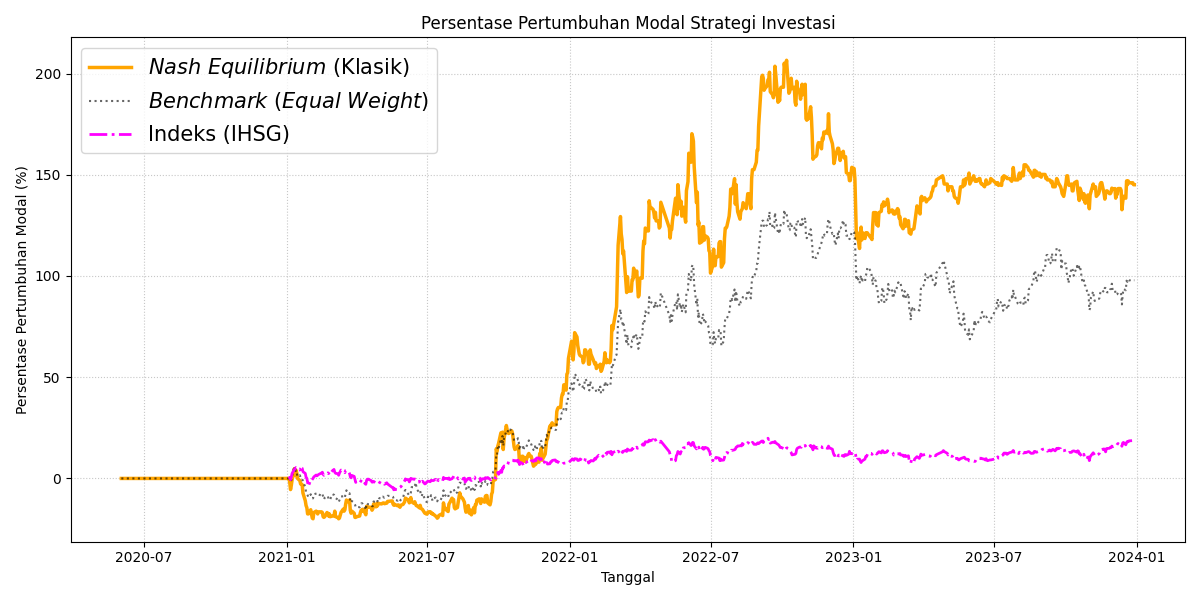
\includegraphics[width=\textwidth]{GTQuantumInvest/Hasil_N2_GT/hasil_backtest_nash_N2.png}
        \caption{Strategi \textit{Nash} (Klasik)}
    \end{subfigure}
    \hfill
    \begin{subfigure}[b]{0.45\textwidth}
        \centering
        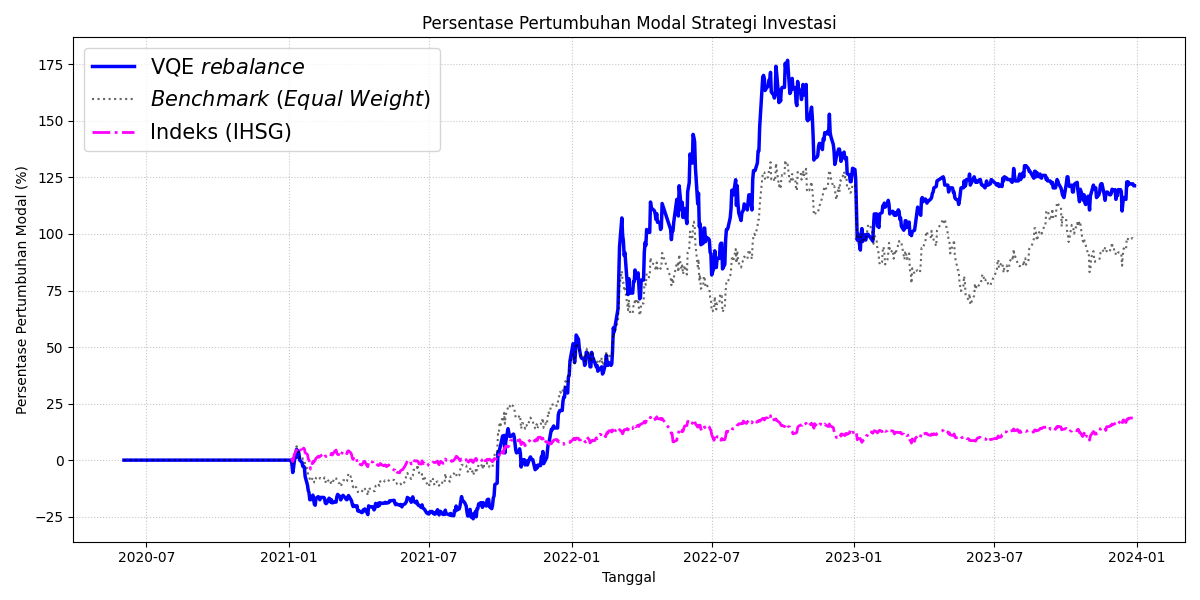
\includegraphics[width=\textwidth]{GTQuantumInvest/Hasil_N2_NoGT/hasil_backtest_vqe_N2.png}
        \caption{VQE (Tanpa \textit{Game Theory})}
    \end{subfigure}
    \caption{Perbandingan Performa Portofolio Klasik vs Kuantum Murni pada Sistem N=2.}
    \label{fig:comp_n2_base}
\end{figure}

\begin{figure}[!htbp]
    \centering
    \begin{subfigure}[b]{0.45\textwidth}
        \centering
        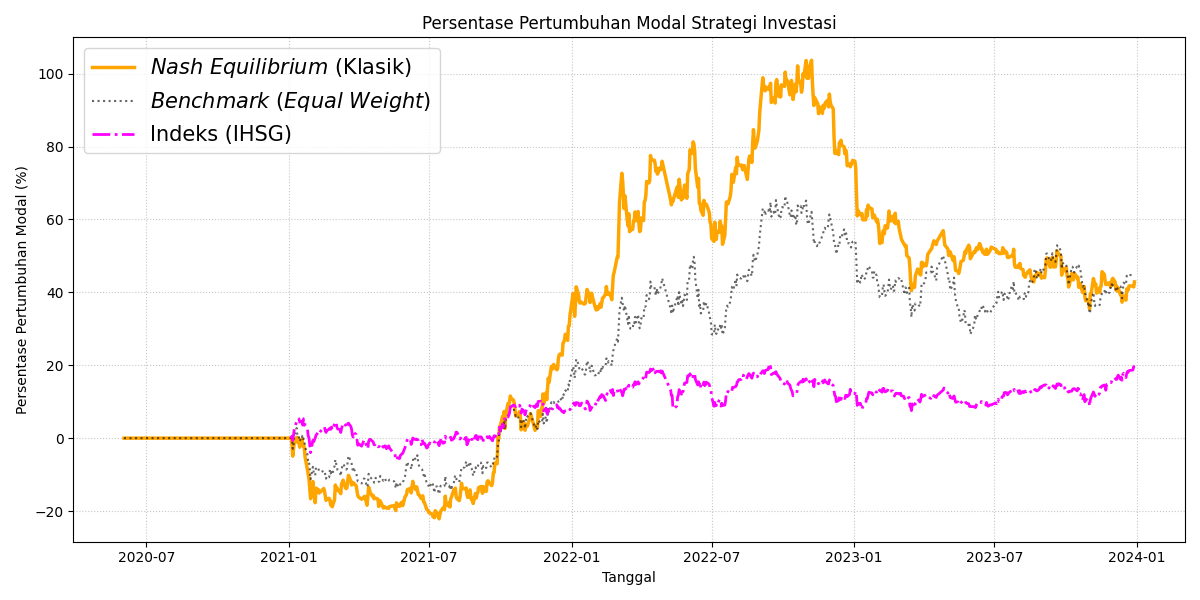
\includegraphics[width=\textwidth]{GTQuantumInvest/Hasil_N4_GT/hasil_backtest_nash_N4.png}
        \caption{Strategi \textit{Nash} (Klasik)}
    \end{subfigure}
    \hfill
    \begin{subfigure}[b]{0.45\textwidth}
        \centering
        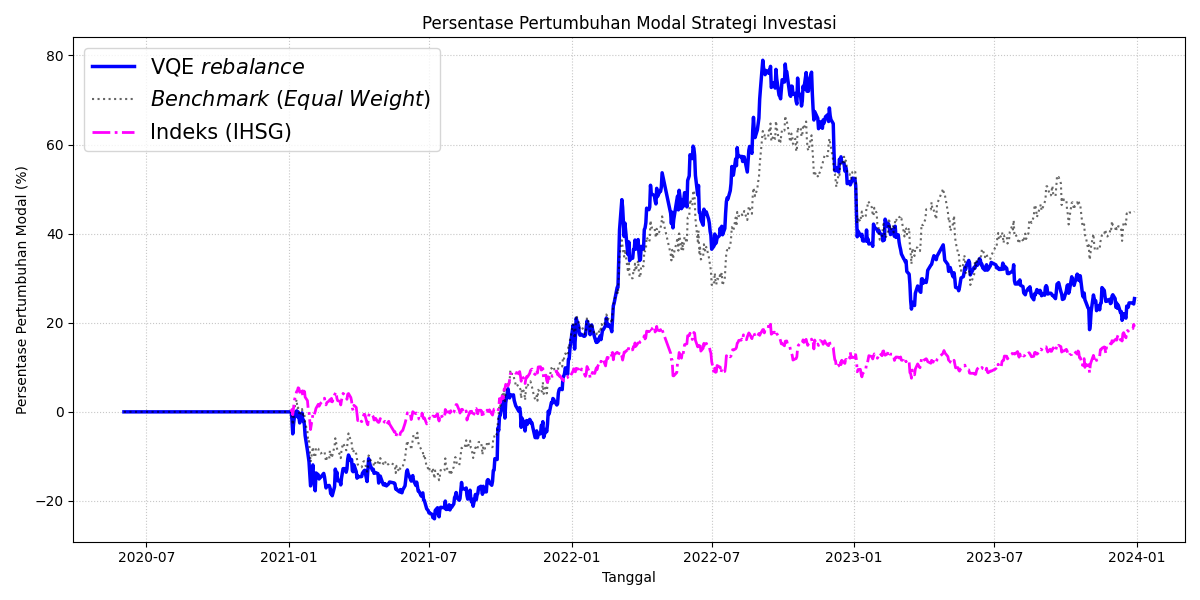
\includegraphics[width=\textwidth]{GTQuantumInvest/Hasil_N4_NoGT/hasil_backtest_vqe_N4.png}
        \caption{VQE (Tanpa \textit{Game Theory})}
    \end{subfigure}
    \caption{Perbandingan Performa Portofolio Klasik vs Kuantum Murni pada Sistem N=4.}
    \label{fig:comp_n4_base}
\end{figure}

Secara kumulatif, efektivitas mekanisme \textit{rebalancing} hibrida ini menghasilkan kurva pertumbuhan modal yang stabil dan \textit{outperform} dari strategi pembandignya. Perbandingan pada Gambar \ref{fig:comp_n2_base} dan \ref{fig:comp_n4_base} menunjukkan bahwa tanpa integrasi kecerdasan strategis, performa VQE murni cenderung tertahan atau bahkan mengalami degradasi saat dimensi sistem membesar. Namun, dengan integrasi \textit{Game Theory} (GT) sebagai inisialisasi keadaan, sirkuit mampu mempertahankan integritas solusinya. Hal ini dapat terbukti juga pada visualisasi Gambar \ref{fig:rebalancing_impact} yang menunjukkan pertumbuhan modal konsisten pada kedua konfigurasi sistem. Oleh karena itu, algoritma ini mampu melindungi nilai portofolio dari potensi (\textit{drawdown}) yang sangat dalam dengan mendeteksi secara dini bagaimana pergeseran ekuilibrium pasar yang terjadi ke dalam dinamika fisis yang dimikiliki oleh sirkuit kuantum.

\begin{figure}[!htbp]
    \centering
    \begin{subfigure}[b]{0.45\textwidth}
        \centering
        
\includegraphics[width=\textwidth]{GTQuantumInvest/Hasil_N2_GT/hasil_backtest_vqe_N2.png}
        \caption{Performa GT-VQE ($N=2$)}
    \end{subfigure}
    \hfill
    \begin{subfigure}[b]{0.45\textwidth}
        \centering
        
\includegraphics[width=\textwidth]{GTQuantumInvest/Hasil_N4_GT/hasil_backtest_vqe_N4.png}
        \caption{Performa GT-VQE ($N=4$)}
    \end{subfigure}
    \caption{Perbandingan Visual Pertumbuhan Modal pada Sistem N=2 dan N=4 sebagai Hasil dari Algoritma \textit{Rebalancing} Strategis.}
    \label{fig:rebalancing_impact}
\end{figure}

